
%(BEGIN_QUESTION)
% Copyright 2014, Tony R. Kuphaldt, released under the Creative Commons Attribution License (v 1.0)
% This means you may do almost anything with this work of mine, so long as you give me proper credit

This bank of pole-mounted power transformers steps 7.2 kVAC line power down to 120/208 VAC power to service a small business:

$$\includegraphics[width=15.5cm]{i00821x01.eps}$$

Given the following power line voltages (measured phase-to-ground), calculate the phase angles of the specified secondary-side voltages:

\begin{itemize}
\item{} $V_U$ = 4160 V $\angle$ $0^o$
\item{} $V_V$ = 4160 V $\angle$ $-120^o$
\item{} $V_W$ = 4160 V $\angle$ $-240^o$
\end{itemize}

\vskip 10pt

\begin{itemize}
\item{} $V_{L1-N}$ = \underbar{\hskip 20pt} $\angle$ \underbar{\hskip 10pt}
\vskip 5pt
\item{} $V_{L2-N}$ = \underbar{\hskip 20pt} $\angle$ \underbar{\hskip 10pt}
\vskip 5pt
\item{} $V_{L3-N}$ = \underbar{\hskip 20pt} $\angle$ \underbar{\hskip 10pt}
\vskip 5pt
\item{} $V_{L1-L3}$ = \underbar{\hskip 20pt} $\angle$ \underbar{\hskip 10pt}
\end{itemize}

\vskip 20pt \vbox{\hrule \hbox{\strut \vrule{} {\bf Suggestions for Socratic discussion} \vrule} \hrule}

\begin{itemize}
\item{} Do these power transformers have {\it additive} or {\it subtractive} polarities?  How can you tell?
\item{} Identify the phase sequence (a.k.a. phase {\it rotation}) of this power system based on the given phase-to-ground power line voltage values.
\end{itemize}

\underbar{file i00821}
%(END_QUESTION)





%(BEGIN_ANSWER)

\noindent
{\bf Partial answer:}

$$\includegraphics[width=15.5cm]{i00821x02.eps}$$

%(END_ANSWER)





%(BEGIN_NOTES)

With each transformer receiving 4160 volts at its primary winding, each secondary winding will output 120 volts at the same phase angle as its corresponding primary phase voltage.  Thus:

\begin{itemize}
\item{} $V_{L1-N}$ = 120 V $\angle$ $0^o$
\vskip 5pt
\item{} $V_{L2-N}$ = 120 V $\angle$ $-120^o$
\vskip 5pt
\item{} $V_{L3-N}$ = 120 V $\angle$ $-240^o$
\end{itemize}

The line voltage $V_{L1-L3}$ may be calculated symbolically by subtracting $V_{L3-N}$ from $V_{L1-N}$:

$$V_{L1-L3} = V_{L1-N} - V_{L3-N}$$

$$V_{L1-L3} = (120 \hbox{ V} \angle 0^o) - (120 \hbox{ V} \angle -240^o)$$

$$V_{L1-L3} = 207.85 \hbox{ V} \angle -30^o$$

The same voltage may be calculated graphically by sketching a phasor $V_{L1-L3}$ between the tips of phasors $V_{L1-N}$ and $V_{L3-N}$:

$$\includegraphics[width=15.5cm]{i00821x02.eps}$$

%INDEX% Electronics review: AC transformer circuit
%INDEX% Electronics review, phasor expressions of circuit quantities
%INDEX% Electronics review, 3-phase transformer bank phase shift calculations

%(END_NOTES)


